\documentclass[../Parameter_fitting.tex]{subfiles}
\graphicspath{{\subfix{../Figures/}}}
\begin{document}
	\sout{The extraction process is assumed to operate in a semi-continuous mode in a cylindrical vessel. The solvent is firstly brought to super-critical condition, pumped through a fixed-bed, of finely chopped biomass, where the solute is extracted from the biomass. Then, the solvent and solute from the extractor are separated in a flush drum, and the extract is collected. The flow rate ($F_{in}$) and inlet temperature ($T_{in}$) of the extractor’s feed can be measured and manipulated. The pressure ($P$) in the vessel can be measured and manipulated, while the outlet temperature ($T_{out}$) can only be measured. A simplified flow diagram is depicted in Figure \ref{fig: SFE_drawing} }.
	
	{\color{blue}The solid-fluid extraction process is assumed to operate in a semi-continuous mode in a cylindrical vessel. In the extractor, essential oils are removed from biomass (for example, carqueja seeds) by supercritical carbon dioxide. As the solvent flows continuously through the bed of porous particles, the $CO_2$ molecules diffuse into the pores and adsorb on the particle surface to form an external fluid film around the solid particles. Then the solute dissolves and diffuses into the solvent in the pores and eventually into the bulk. The solvent-solute mixture leaves the extractor and undergoes depressurization. The $CO_2$ is released to a gaseous state, and the solute precipitates. In the vapour-liquid separator, the gaseous solvent is vent off while the precipitated product is collected.
		
		In Figure \ref{fig: SFE_drawing}, an instrumental set-up is presented. The flow rate ($F_{in}$) and the temperature ($T_{in}$) of the solvent entering the extractor are measured and can be adjusted using a pump and a heat exchanger, respectively. Moreover, the extractor's pressure ($P$) is assumed to be measurable and adjustable using a back-pressure regulator valve. In addition, the temperature of the outlet stream $T_{out}$ and the temperature profile of the fixed-bed can be measured. }
	
	\begin{figure}[h]
		\centering
		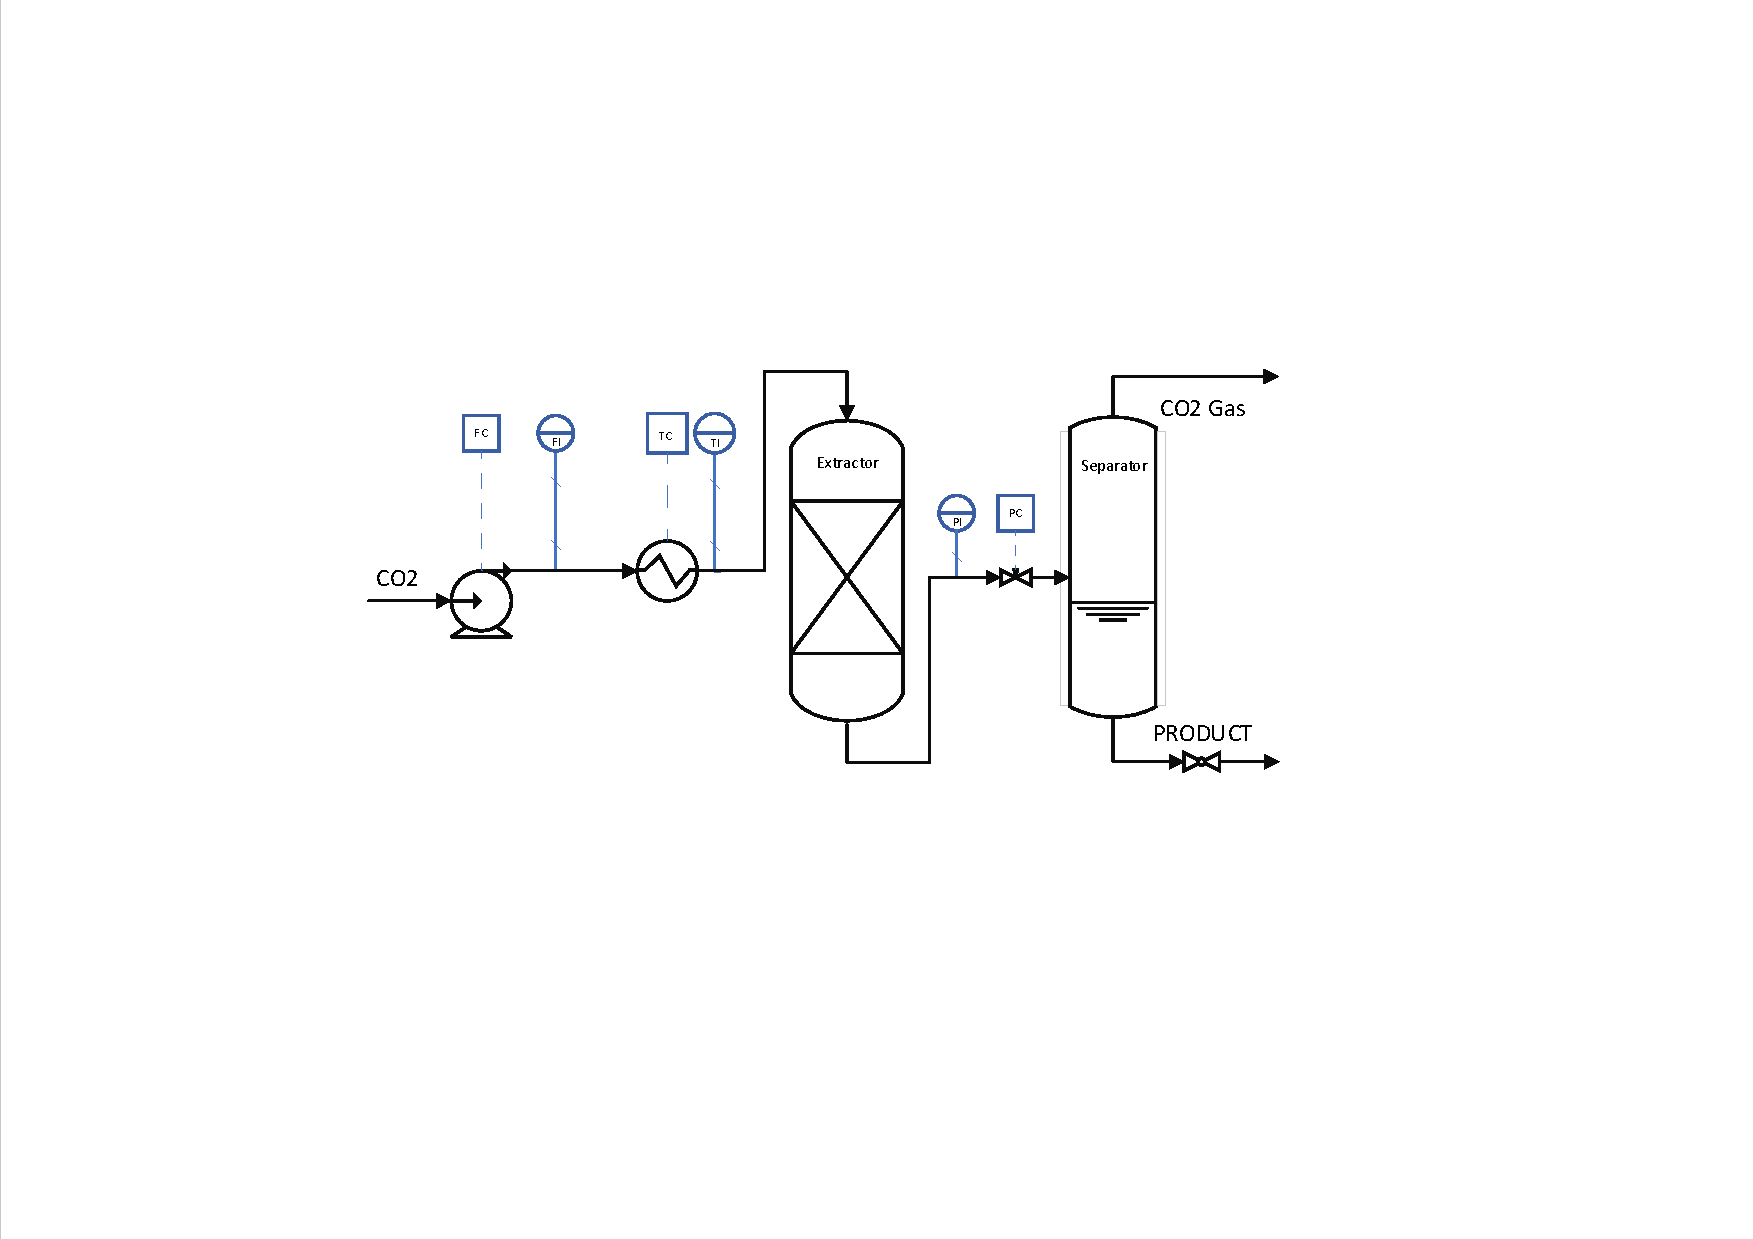
\includegraphics[trim = 6cm 7.5cm 8cm 6cm, clip, width=\linewidth]{SFE_PFD.pdf}
		\caption{Process flow diagram for solid-fluid extraction process}
		\label{fig: SFE_drawing}
	\end{figure}

\end{document}